\documentclass[12pt]{article}
\usepackage[margin=0.8in]{geometry}
\usepackage{colortbl}
\usepackage{placeins}
\usepackage{graphicx}
\usepackage{listings}
\usepackage[usenames,dvipsnames]{xcolor}
\usepackage{xcolor}
\pagecolor{white}
\definecolor{dkgreen}{rgb}{0,0.6,0}
\definecolor{gray}{rgb}{0.5,0.5,0.5}
\definecolor{mauve}{rgb}{0.58,0,0.82}

\lstset{frame=tb,
  language=Java,
  aboveskip=3mm,
  belowskip=3mm,
  showstringspaces=false,
  columns=flexible,
  basicstyle={\small\ttfamily},
  numbers=none,
  numberstyle=\tiny\color{gray},
  keywordstyle=\color{blue},
  commentstyle=\color{dkgreen},
  stringstyle=\color{mauve},
  breaklines=true,
  breakatwhitespace=true,
  tabsize=3
}

\usepackage{hyperref}
\usepackage{subcaption}
\usepackage{amssymb}
%% The amsthm package provides extended theorem environments
\usepackage{amsthm}
\usepackage{amsmath}
\title{\color{BlueViolet}\bfseries\Huge Calculating Heating by the Electron Beam In an Fe Foil}
\author{\color{BurntOrange}donald.jones@temple.edu}
\date{}
\begin{document}
\maketitle
This technical note TargetHeating.tex, TargetHeating.pdf and the accompanying code FeFoilHeating.C can be found in the following Github repository: \\https://github.com/jonesdc76/MollerPolarimetry/tree/master/TargetPolarization
\section{Solving the Heat Equation Specific to the Hall A M\o ller Polarimeter}
To calculate the heating of the M\o ller polarimeter iron foil we start with the heat equation. Given the geometry of the M\o ller foil where we have a circular10~$\mu$m thick foil with a beam heat source located at the center, we can assume this has no azimuthal or z-dependence and we are left with only a radial dependence:
\begin{equation}
\label{eq:heat_T_r_t}
\rho C_p\frac{\partial T}{\partial t}=\kappa\nabla^2T+\rho\alpha B_{flux}-\frac{2\sigma\epsilon}{\Delta z}\left(T^4-T_0^4\right).
\end{equation}
\begin{itemize}
\item{$T(r, t)$ is the foil temperature in Kelvin,}
\item{$\kappa$ is the temperature dependent thermal conductivity of Fe which is approximately 0.8~W/(K cm) at room temperature,}
\item{$\rho =7.87$~g/cm$^3$ is the density of Fe,}
\item{$\sigma =5.67\times 10^{-12}$~W/(K$^4$ cm$^2$) is the Stefan-Boltzmann constant,}
\item{$\epsilon$ is the foil emissivity which depends on the polish and structure of the surface ranging from 0 (perfect polish) to 1 (perfect blackbody). Given the polish of the foil, something like 0.1 can be assumed.}
\item{$T_0=294$~K, is the ambient temperature of the target ladder holding the foil at its boundary,}
\item{$\Delta z=10~\mu$m is the thickness of the foil,}
\item{$\alpha$ is the collision stopping power for electrons in Fe. It is a function of electron energy and is 2.043~(MeV cm$^2$)/g$=$3.273$\times 10^{-13}$(J cm$^2$)/g for a 10~GeV electron using ESTAR. The ESTAR data along with a 5-degree polynomial fit used to calculate $\alpha$ as a function of energy is shown in Fig. \ref{fig:stopping}. Care should be exercised when extrapolating outside the 1-10~GeV range.}
\item{$C_p=0.45$~J/(g K) is the specific heat of Fe and,} 
\item{$B_{flux}=\frac{d^3N_e}{ds dt} $ is the flux density of the beam in $e^-$/(cm$^2$ s).}
\end{itemize}
\begin{figure}[h]
\centering
\includegraphics[width=0.9\linewidth]{StoppingPower.png}
\caption{\label{fig:stopping}Stopping power for electrons as a function of energy in Fe. Data are from ESTAR and are fit to a 5-degree polynomial.}
\end{figure}
In principle $T$ and $B_{flux}$ are functions of position and time. However, we are interested in the temperature of the steady state which is presumably reached quite rapidly when the beam turns on. Setting $\frac{\partial T}{\partial t}=0$ simplifies Eq. \ref{eq:heat_T_r_t}. The expected heat load on a $10~\mu$m thick Fe foil in the electron beam is about 12~mW/$\mu$A. If the temperature increase with beam inside the beam flux is of 30 degrees Celsius or less, over a beam radius of 1~mm, then the radiated energy in this circular area is 0.13~mW or about 1\% of the heat load. In this case, we can safely neglect the radiative cooling term. If we end up with a temperature increase greater than 30 degrees, then we will have to revisit this assumption. Under these assumptions, Eq. \ref{eq:heat_T_r_t} simplifies to  
\begin{align}
\kappa\nabla^2T&=-\rho\alpha B_{flux}\\
\frac{\kappa}{r}\frac{\partial}{\partial r}\left(r\frac{\partial T}{\partial r}\right)&=-\rho\alpha B_{flux}\\
\label{eq:heat_T_r}
\frac{\partial}{\partial r}\left(r\frac{\partial T}{\partial r}\right)&=-\frac{\rho\alpha}{\kappa}rB_{flux}.
%\frac{\partial}{\partial r}\left(r\frac{\partial T}{\partial r}\right)&=\gamma rB_{flux}\,\
\end{align}
%where $\gamma\equiv\rho\alpha/\kappa$.
The Hall A M\o ller polarimeter, does not typically take rastered beam, and it is thus reasonable to assume a Gaussian beam flux profile of radius $r_b$. Therefore, the Gaussian profiled electron flux $B_{flux}$ from a beam current $I$ in Amperes with a $1~\sigma$ radius of $r_{b}$ becomes
\begin{equation}
B_{flux}=\frac{I}{1.6\times 10^{-19} \left(2\pi r_{b}^2\right)}e^{-r^2/2r_b^2}.
\end{equation}
Inserting this density profile for the electron beam heat source into Eq. \ref{eq:heat_T_r} gives
\begin{equation}
\label{eq:heat_Tr_simp}
\frac{\partial}{\partial r}\left(r\frac{\partial T}{\partial r}\right)=-\gamma re^{-r^2/2r_b^2},
\end{equation} 
where $\gamma\equiv\frac{I\rho\alpha}{1.6\times 10^{-19} \kappa\left(2\pi r_{b}^2\right)}$.
Integrating both sides of Eq. \ref{eq:heat_Tr_simp} w.r.t. $r$ gives
\begin{align}
r\frac{\partial T}{\partial r}&=r_b^2\gamma e^{-r^2/2r_b^2}+C,\\
\label{eq:Tslope}
\frac{\partial T}{\partial r}&=\frac{r_b^2\gamma}{r} e^{-r^2/2r_b^2}+\frac{C}{r}
\end{align} 
where $C$ is a constant of integration to be determined from boundary conditions in the steady state. To determine $C$, the total heat load from the beam is given by $I\alpha\rho\Delta z/1.6\times10^{-19}=11.8\Delta z$~W/($\mu$A~cm). The heat flow through the boundary is the product of the conductivity $\kappa$, the cross sectional area of the foil along the foil perimeter $2\pi R_{foil}\Delta z$ and the temperature slope $\partial T /\partial r$, where  length units are in cm. The perimeter of the foil at $R_{foil}$ is assumed to be kept fixed at room temperature. The heat flow at the boundary has to equal the beam heat load in the steady state, so 
\[
\left(\kappa2\pi R_{foil}\Delta z\right) \frac{\partial T}{\partial r}|_{r=R_{foil}}\approx-11.8\Delta z\left(\frac{\textrm{W}}{\mu \textrm{A cm}}\right)\approx\frac{\left(\kappa2\pi R_{foil}\Delta z\right) C}{R_{foil}},
\]
where the first term on the left side of Eq. \ref{eq:Tslope}) is not included since it is negligible at the boundary of the foil $R_{foil}$. The negative sign comes from the direction of heat flow towards higher radius making the temperature decrease with increasing $r$.
\[
C\approx-\frac{11.8}{2\pi\kappa}=-2.50\left(\frac{\textrm{K}}{\mu\textrm{A}}\right),
\]
where the value for Fe has been used $\kappa=$0.75~W/(K cm). Now to find the temperature difference between the outside perimeter of the foil at $r=R_{foil}$ and some $r<R_{foil}$ integrate both sides from $R_{foil}$ to $r$ yielding
\begin{equation}
\label{eq:dT}
\Delta T = \int_{R_{foil}}^r \left(\frac{r_b^2\gamma}{r^{\prime}} e^{-r^{\prime 2}/2r_b^2}+\frac{C}{r^{\prime}}\right)dr^{\prime}.
\end{equation}
This can easily be integrated numerically as shown in Figures  \ref{fig:foilheating} and \ref{fig:foilheatingT}.
\begin{figure}[h]
\centering
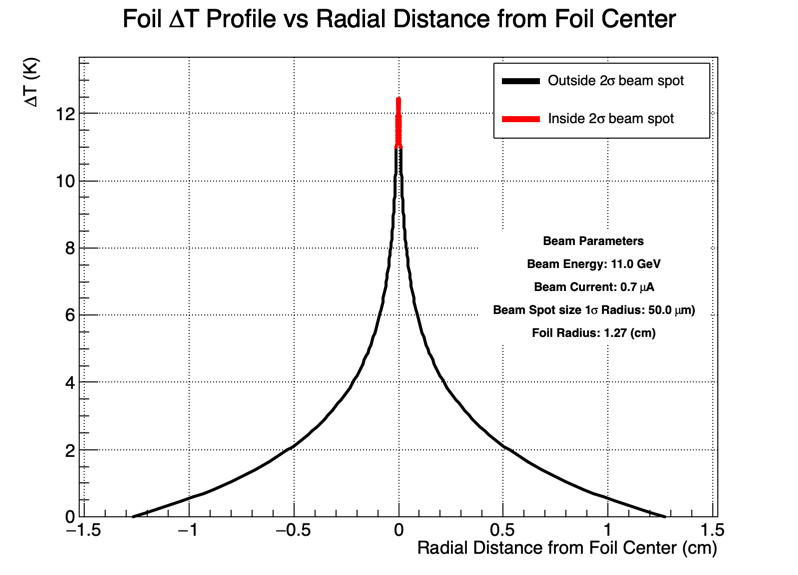
\includegraphics[width=0.9\linewidth]{FoilHeatingdT.png}
\caption{\label{fig:foilheating}Fe foil $\Delta T$ profile from integrating Eq. \ref{eq:dT} with beam spot size, and energy given. For this example, the foil and beam parameters are approximately used during PREX/CREX.}
\end{figure}
\begin{figure}[h]
\centering
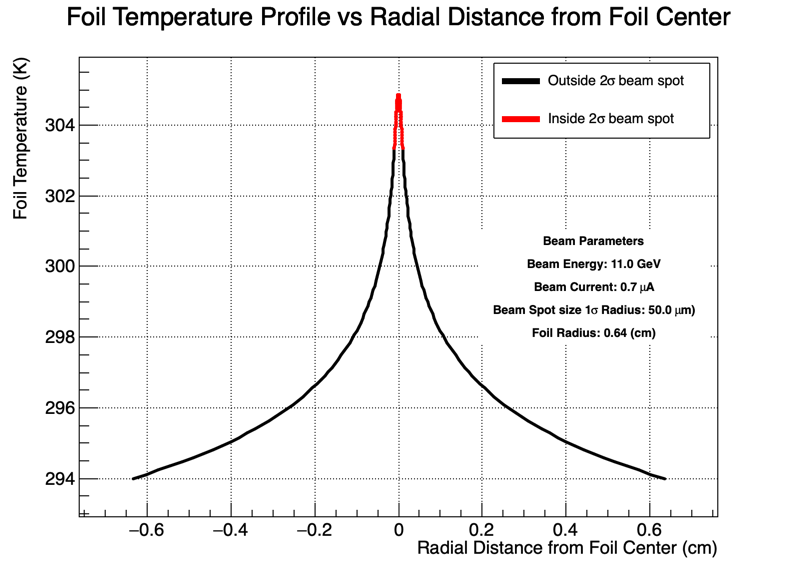
\includegraphics[width=0.9\linewidth]{FoilHeatingT.png}
\caption{\label{fig:foilheatingT}Fe foil temperature profile from integrating Eq. \ref{eq:dT} with beam spot size, and energy given. For this example, the foil and beam parameters are approximately used during PREX/CREX.}
\end{figure}

\FloatBarrier
\newpage
\section{C++/ROOT Code for Numerically Integrating Eq. \ref{eq:dT}}
The following ROOT macro uses Eq. \ref{eq:dT} to calculate the foil heating for a circular Fe foil in a Gaussian profile electron beam.
\begin{lstlisting}
#include "TF1.h"
#include <iostream>
#include "TGraph.h"
#include "TLegend.h"
#include "TAxis.h"
#include "TPad.h"
#include "TCanvas.h"
#include "TStyle.h"
#include "TPaveText.h"
#include "TString.h"

///////////////////
//Donald C. Jones//
//Nov. 2021        //
///////////////////

//////////////////////////////////////////////////////////////////////
//FeFoilHeating() calculates and graphs the temperature difference 
//in a thin circular  Fe foil between its edge held at a fixed 
//temperature T0 and inside a circular  Gaussian-distributed 
//electron beam.                                                 
//     
//                                                                               
//Arguments:                                                                         
//  beam_cur: beam current in Amperes                                                
//  beam_r:    1 sigma beam spot size radius in cm                                    
//  beam_E:    beam energy in GeV                                                      
//  T0:        ambient (Hall) temperature in Kelvin taken as foil 
//             boundary temperature 
//                                                                              
//Returns the foil temperature difference in degrees K between T0
//at the foil edge and the temperature at the 1-sigma beam 
//radius r_beam.       
//                       
//NOTE: it is helpful to recall that for a 2D circular Gaussian 
//distribution the volume between r=0 and the n-sigma points 
//are as follows:                           
//1sigma = 39.35%,  2sigma = 86.47%, 3sigma = 98.89%, 4sigma = 99.97%
//Therefore, the temperature should be averaged over at least 3 sigma.    
/////////////////////////////////////////////////////////////////////////

double FeFoilHeating(double beam_cur = 1e-6, double beam_r=5e-3, 
                       double beam_E = 11, double T0 = 294){
  gStyle->SetStatY(0.7);
  gStyle->SetStatH(0.2);
  gStyle->SetOptFit(1111);
  gStyle->SetTitleW(0.95);


  const double rho = 7.87;//density of Fe
  const double sigma = 5.670e-12;//Stefan Boltzman constant W/(cm^2 K^4)
  const double Cp = 0.45;//Fe specific heat capacity in J/(g K)
  const double echarge = 1.602e-19;//Coulombs per electron
  const double R_foil = 0.5*2.54/2.0;//radius of Fe foil in cm
  const double PI = 3.1415927;//pi obviously

  

  //Use ESTAR data to estimate energy loss as a function of electron energy
  //----------------------------------------------------------------------------------
  TCanvas *c = new TCanvas("c","c",0,0,800,600);
  double beam_en[10]={1,2,3,4,5,6,7,8,9,10};//beam energy in GeV
  double stop_en[10]={1.878,1.928,1.957,1.977,1.993, //collision stopping power 
		      2.006,2.017,2.027,2.035,2.043};//in (MeV cm^2/g) using ESTAR
  TGraph *grStop = new TGraph(10,beam_en,stop_en);
  grStop->SetTitle("Electron Stopping Power for Fe vs Beam Energy (ESTAR Data)");
  grStop->SetMarkerStyle(8);
  grStop->Draw("ap");
  grStop->GetXaxis()->SetTitle("Electron Energy");
  grStop->GetYaxis()->SetTitle("Stopping Power (MeV cm^{2}/g)");
  gPad->Update();
  TF1 *fStop = new TF1("fStop","pol5",0,1);//use fit to give continuous function
  grStop->Fit(fStop);  
  double alpha = echarge*fStop->Eval(beam_E)*1e6;//Collision stopping power in (Jcm^2/g)
  cout<<"Stopping power "<<alpha<<" (J cm^2/g)"<<endl;
  c->SaveAs("StoppingPower.png");

  

  //Calculate the energy dependent thermal conductivity of Fe using data either from
  //https://www.efunda.com/materials/elements/TC_Table.cfm?Element_ID=Fe
  //or
  //https://www.engineeringtoolbox.com/thermal-conductivity-metals-d_858.html
  //----------------------------------------------------------------------------------
  bool data_efunda = 1;
  TCanvas *ct = new TCanvas("ct","ct",0,0,800,600);
  double temp[4] = {250,300,350,400};
  double cond[4] = {0.865,0.802,0.744,0.695};//www.efunda.com
  TGraph *grC = new TGraph(4,temp,cond);
  grC->SetTitle("Fe Thermal Conductivity vs. Temperature");
  grC->SetMarkerStyle(8);
  grC->Draw("ap");
  grC->GetXaxis()->SetTitle("Temperature (k)");
  grC->GetYaxis()->SetTitle("Thermal Conductivity (W/cm K)");
  TF1 *fCond = new TF1("fCond","pol2",0,1);
  grC->Fit(fCond);
  gPad->Update();
  if(!data_efunda)//www.engineeringtoolbox.com
    fCond = new TF1("fCond","0.835-0.001102*(x-273)",0,1);
  double guessTemp = T0+15*beam_cur/1e-6;//starting guess for final foil temperature
  double kappa = fCond->Eval(guessTemp);
  cout<<"Conductivity at "<<guessTemp<<" K is "<<kappa<<endl;
  ct->SaveAs("FeThermalCond.png");


  
  //Integral of f(r) gives delta T. Create the integrand f(r) 
  //----------------------------------------------------------------------------------
  double gam = beam_cur/echarge*rho*alpha/kappa/2./PI/pow(beam_r,2);
  double C = -beam_cur/echarge*alpha*rho/2.0/PI/kappa;
  TF1 *f = new TF1("f",Form("%e/x*exp(-x*x/%e)+%e/x",
			    beam_r*beam_r*gam,2*beam_r*beam_r,C),0,R_foil);


  
  //Improve thermal conductivity estimate using the calculated temperature.
  //Temperature at 1.3*beam_r is a good estimate of the average temperature
  //weighted by the beam spot charge distribution.
  //-----------------------------------------------------------------------------------
  guessTemp = f->Integral(R_foil,1.3*beam_r)+T0;
  kappa = fCond->Eval(guessTemp);
  gam = beam_cur/echarge*rho*alpha/kappa/2./PI/pow(beam_r,2);
  C = -beam_cur/echarge*alpha*rho/2.0/PI/kappa;
  cout<<"Conductivity re-calculated at "<<guessTemp<<" K is "<<kappa<<endl;
  f = new TF1("f",Form("%e/x*exp(-x*x/%e)+%e/x",beam_r*beam_r*gam,2*beam_r*beam_r,C),0,R_foil);



  //Graph resulting temperature profile by integrating f(r)dr. Make points red inside
  //2 sigma beam spot size radius.
  //-----------------------------------------------------------------------------------
  const int N=500;
  double r[N], T[N], dT[N],ri[N],Ti[N], dTi[N];
  int n=0, ni=0;
  double rp = R_foil;
  for(int i=0;i<N/2;++i){
    r[i]=rp;
    dT[i] = f->Integral(R_foil,rp);
    T[i] = dT[i]+T0;
    if(rp<2*beam_r){
      ri[ni]=rp;
      Ti[ni]=T[i];
      dTi[ni]=dT[i];
      ++ni;
    }
    rp*=0.95;
    ++n;
    if(rp<0.00001)break;
  }
  for(int i=0;i<n;++i){
    r[i+n]=-r[n-i-1];
    dT[i+n] = dT[n-i-1];
    T[i+n] = T[n-i-1];
  }
  for(int i=0;i<ni;++i){
    ri[i+ni]=-ri[ni-i-1];
    dTi[i+ni] = dTi[ni-i-1];
    Ti[i+ni] = Ti[ni-i-1];
  }
  TCanvas *c1 = new TCanvas("c1","c1",0,0,800,600);
  TGraph *grdT = new TGraph(2*n,r,dT);
  grdT->SetMarkerStyle(8);
  grdT->SetLineWidth(6);
  grdT->SetMarkerSize(0.3);
  grdT->Draw("acp");
  grdT->SetTitle(Form("Foil #DeltaT Profile vs Radial Distance from Foil Center"));
  grdT->GetXaxis()->SetTitle("Radial Distance from Foil Center (cm)");
  grdT->GetYaxis()->SetTitle("#DeltaT (K)");
  TGraph *gridT = new TGraph(2*ni,ri,dTi);
  gridT->SetMarkerStyle(8);
  gridT->SetMarkerColor(kRed);
  gridT->SetLineColor(kRed);
  gridT->SetLineWidth(6);
  gridT->SetMarkerSize(0.4);
  gridT->Draw("samecp");
  gPad->SetGrid();
  TPaveText *pt = new TPaveText(0.6,0.4,0.89,0.6,"ndc");
  pt->SetFillColor(0);
  pt->SetShadowColor(0);
  pt->SetBorderSize(0);
  pt->AddText("Beam Parameters");
  pt->AddText(Form("Beam Energy: %0.1f GeV",beam_E));
  pt->AddText(Form("Beam Current: %0.1f #muA", beam_cur*1e6));
  pt->AddText(Form("Beam Spot size 1#sigma Radius: %0.1f #mum)",beam_r*1e4));
  pt->AddText(Form("Foil Radius: %0.2f (cm)",R_foil));
  pt->Draw();
  TLegend *lg = new TLegend(0.62,0.76,0.89,0.89);
  lg->AddEntry(grdT,"Outside 2#sigma beam spot","lp");
  lg->AddEntry(gridT,"Inside 2#sigma beam spot","lp");
  lg->Draw();
  c1->SaveAs("FoilHeatingdT.png");
  TCanvas *c2 = new TCanvas("c2","c2",0,0,800,600);
  TGraph *gr = new TGraph(2*n,r,T);
  gr->SetMarkerStyle(8);
  gr->SetLineWidth(6);
  gr->SetMarkerSize(0.3);
  gr->Draw("acp");
  gr->SetTitle(Form("Foil Temperature Profile vs Radial Distance from Foil Center"));
  gr->GetYaxis()->SetTitle("Foil Temperature (K)");
  gr->GetXaxis()->SetTitle("Radial Distance from Foil Center (cm)");
  TGraph *gri = new TGraph(2*ni,ri,Ti);
  gri->SetMarkerStyle(8);
  gri->SetMarkerColor(kRed);
  gri->SetLineColor(kRed);
  gri->SetLineWidth(6);
  gri->SetMarkerSize(0.4);
  gri->Draw("samecp");
  gPad->SetGrid();
  lg->Draw();
  pt->Draw();
  c2->SaveAs("FoilHeatingT.png");

  

  //Integrate f(r) weighted by the beam charge distribution to find average delta T 
  //-----------------------------------------------------------------------------------
  gStyle->SetOptFit(0);
  TF1 *fGaus = new TF1("fGaus","[0]*exp(-x*x/(2*[1]*[1]))+[2]",-2*beam_r,2*beam_r);
  fGaus->SetParameters(guessTemp/2.,beam_r,T0);
  gr->Fit(fGaus,"r");
  TString func = Form("(%e*exp(-x*x/(2*%e))+%e)*x*exp(-x*x/2./%e)/%e",
		      fGaus->GetParameter(0),pow(fGaus->GetParameter(1),2),
		      fGaus->GetParameter(2),beam_r*beam_r,beam_r*beam_r);
  TF1 *fAvgT = new TF1("fAvgT",func.Data(),0,1);
  fAvgT->SetNpx(1000);
   //fAvgT->Draw();
  cout<<"dT at 1.3 sigma is "<<f->Integral(R_foil,beam_r*1.3)<<endl;

  

  //Return average temperature, weighted by the beam spot charge distribution.
  //-----------------------------------------------------------------------------------
  return fAvgT->Integral(0,10*beam_r);
}
\end{lstlisting}
\end{document}
